%----------------------------------------------------------------------------- %%
\section{Policy Design and Implementation}
\label{bab:3}
%----------------------------------------------------------------------------- %%

This section presents the design and implementation of \textit{ResourceDefragmentation}, a \textit{Balance} plugin for post-placement consolidation in the Kubernetes Descheduler. It builds a snapshot of worker Nodes based on Pod resource requests, finds source Nodes that are either sparse or poorly shaped in CPU-memory space, predicts feasible landing Nodes for their Pods, and evicts the Pod whose predicted scheduler target has the strongest projected CPU-memory bin score. The kube-scheduler remains responsible for final binding.

The experimental configuration explicitly uses declared Pod requests. This keeps Node assessment, feasibility checks, and target prediction aligned with the admission model used by kube-scheduler, and it deliberately excludes runtime (actual) usage so that placement feasibility and bin-packing shape drive every decision.

\subsection{System Overview}
\label{sec:defrag_system_overview}

Figure~\ref{fig:defrag_highlevel} shows the end-to-end control flow of the \textit{ResourceDefragmentation} plugin, from the entry point of the Descheduler \textit{Balance} function to the eviction decision. The plugin operates in two phases: an assessment-and-ordering phase that builds the drain-candidate set, and a bounded eviction loop that relocates Pods from those candidates.

In the first phase, the plugin scans every worker Node. Control-plane Nodes are skipped, and for each remaining Node it computes the average utilization and bin score. A Node whose average utilization and bin score both stay at or above the drain threshold is well-packed and is skipped; otherwise the Node is scored with its Resource Imbalance Index (RII), Free-Space Index (FSI), and priority \(P_n\), added to the drain-candidate set, and the set is sorted in descending priority.

In the second phase, the plugin iterates over the ordered candidates. The loop stops once the per-sweep eviction budget is reached. A Node already marked as a bin, that is, a recent eviction target, is skipped so the same sweep does not drain a Node it has just packed. Otherwise the plugin selects the Pod whose predicted scheduler target has the highest projected bin score; if a feasible target exists the Pod is evicted and the local cache and bin set are updated, and if not the Node is skipped. The remaining subsections formalize each stage: Section~\ref{sec:defrag_node_metrics} defines the Node-state metrics, Section~\ref{sec:defrag_drain_candidates} the drain-candidate detection and ordering, Section~\ref{sec:defrag_target_prediction} the predicted scheduler target, and Section~\ref{sec:defrag_victim_selection} the eviction-candidate selection.

\begin{figure*}[tbp]
    \centering
    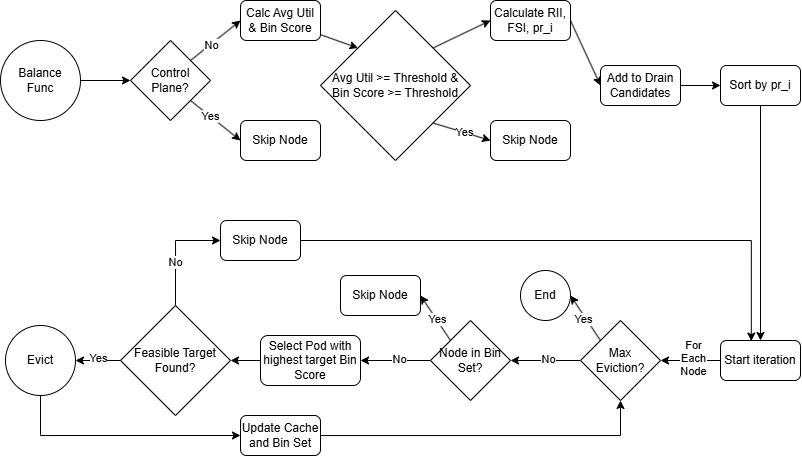
\includegraphics[width=0.95\textwidth]{assets/pics/defrag/highlevel_defrag.png}
    \caption{High-level control flow of the \textit{ResourceDefragmentation} plugin, from Node assessment and drain-candidate ordering to the bounded predicted-target eviction loop.}
    \label{fig:defrag_highlevel}
\end{figure*}

\subsection{Node-State Metrics}
\label{sec:defrag_node_metrics}

For Node \(n\), let \(u_{n,c}\) and \(u_{n,m}\) denote normalized requested CPU and memory:

\[
    u_{n,c} = \frac{R_{n,c}}{C_{n,c}},
    \qquad
    u_{n,m} = \frac{R_{n,m}}{C_{n,m}},
\]

where \(u_{n,c}\) is the normalized CPU utilization of Node \(n\), \(u_{n,m}\) is the normalized memory utilization of Node \(n\), \(R_{n,c}\) is the sum of CPU requests from all Pods on Node \(n\), \(R_{n,m}\) is the sum of memory requests from all Pods on Node \(n\), \(C_{n,c}\) is the allocatable CPU capacity of Node \(n\), and \(C_{n,m}\) is the allocatable memory capacity of Node \(n\). Average utilization represents density:

\[
    U_n^{avg} = \frac{u_{n,c} + u_{n,m}}{2},
\]

where \(U_n^{avg}\) is the average utilization of Node \(n\), representing overall resource density by taking the mean of normalized CPU and memory utilization.

The bin score is a custom composite scoring function derived from the standard multi-dimensional bin-packing heuristics used in the Kubernetes scheduling plugins~\cite{k8s_resource_bin_packing}. It fuses two signals that those plugins apply separately, namely the density preference of the \texttt{MostAllocated} strategy, which favors well-filled Nodes, and the per-dimension balance preference of the \texttt{BalancedAllocation} strategy, which penalizes Nodes whose CPU and memory utilization diverge. Combining density and dimensional balance into a single quantity yields

\[
    B_n =
    \frac{
        \frac{u_{n,c}+u_{n,m}}{2}
        \left(1-\left|u_{n,c}-u_{n,m}\right|\right)
    }{2},
\]

where \(B_n\) is the bin score of Node \(n\). The first factor \(\tfrac{u_{n,c}+u_{n,m}}{2}\) is the density term inherited from \texttt{MostAllocated}, while the penalty factor \(1-|u_{n,c}-u_{n,m}|\) is the balance term inherited from \texttt{BalancedAllocation}, which reduces the score when CPU and memory utilization diverge. A dense and balanced Node therefore has a high \(B_n\), whereas an empty or strongly skewed Node has a lower score. The signed Resource Imbalance Index, adapted to normalized request fractions from the server imbalance index of \cite{guo2025joint}, identifies the skew direction:

\[
    RII_n = u_{n,c} - u_{n,m},
\]

where \(RII_n\) is the Resource Imbalance Index of Node \(n\). A positive value indicates CPU-heavy skew (CPU utilization exceeds memory utilization), while a negative value indicates memory-heavy skew. The Free-Space Index, adapted from the free-space size index of \cite{guo2025joint} by expressing the headroom in normalized rather than absolute units, represents joint CPU-memory headroom:

\[
    FSI_n = (1-u_{n,c})(1-u_{n,m}),
\]

where \(FSI_n\) is the Free-Space Index of Node \(n\), representing the product of remaining CPU capacity \((1-u_{n,c})\) and remaining memory capacity \((1-u_{n,m})\). A higher \(FSI_n\) indicates a larger jointly usable headroom region, while a low \(FSI_n\) suggests constrained free space in at least one dimension.

\subsection{Drain-Candidate Detection and Ordering}
\label{sec:defrag_drain_candidates}

A worker Node with at least one evictable Pod becomes a drain candidate when either its average utilization or its bin score is below the configured drain threshold \(\tau\):

\[
    U_n^{avg} < \tau
    \quad \lor \quad
    B_n < \tau.
\]

The disjunction allows the policy to act on two resource-only states. A lightly utilized but balanced Node can be drained to free infrastructure, while a more utilized but badly skewed Node can be drained because its remaining headroom is hard to reuse.

Drain candidates are processed in descending priority:

\[
    P_n =
    0.5\left|RII_n\right|
    +
    0.5\frac{1}{FSI_n+1\mathrm{e}{-}10}.
\]

The first term emphasizes dimensional skew. The second term emphasizes a narrow jointly usable free-space region. Following the priority formulation of \cite{guo2025joint}, the constant is fixed at \(1\mathrm{e}{-}10\) and is added to the free-space term of \emph{every} Node as a numerical guard against division by zero, rather than being applied conditionally only when \(FSI_n = 0\). Because \(1\mathrm{e}{-}10\) is negligible relative to any non-zero \(FSI_n \in (0,1]\), it leaves the relative ordering of drain candidates unchanged for partially loaded Nodes, while bounding the term to a large finite value of \(1\mathrm{e}{+}10\) when a Node has no jointly usable headroom (\(FSI_n = 0\)), so that fully constrained Nodes receive the highest priority. Utilization and bin score decide whether a Node enters the drain set, while RII and FSI decide which drain candidate is handled first.

The two weights of \(0.5\) generalize the priority formulation of \cite{guo2025joint}, which writes the priority as \(w_p\left|RII_n\right| + (1-w_p)\,/(FSI_n+\epsilon)\) for a tunable weight \(w_p\). Setting \(w_p = 0.5\) treats dimensional skew and free-space scarcity as co-equal fragmentation signals, so that neither criterion is privileged a priori in the absence of a workload-specific reason to favor one. The two terms nonetheless occupy different numeric ranges: \(\left|RII_n\right| \in [0,1]\), whereas \(1/(FSI_n+1\mathrm{e}{-}10) \in [1,\,1\mathrm{e}{+}10]\). The free-space term therefore dominates the ordering for densely packed Nodes that have little joint headroom, while \(\left|RII_n\right|\) acts as a secondary, skew-based tie-breaker among Nodes with comparable free space.

Adjusting this weighting does not change the descheduler as a whole. The priority \(P_n\) governs only the \emph{order} in which already-selected drain candidates are processed; it does not decide which Nodes enter the drain set, whether a predicted target is feasible, the pack-upward guard, the utilization ceiling, or the bounded convergence loop. Re-weighting therefore alters the drain trajectory, namely which Node is handled first and possibly the number of passes required, and can shift the final layout only at the margin, for instance when the pass budget is exhausted before convergence. Because every pass re-evaluates the cluster state and the loop terminates only when a pass produces zero evictions, the policy's feasibility, safety, and convergence properties are independent of \(w_p\), and the converged layout remains stable across reasonable weightings. The weight is thus a tuning knob for ordering and efficiency rather than a parameter that redefines what the descheduler is permitted to evict.

\subsection{Predicted Scheduler Target}
\label{sec:defrag_target_prediction}

For every evictable Pod \(p\) on source Node \(s\), the plugin examines each non-origin worker Node as a potential relocation target. Let \(r_{p,c}\) and \(r_{p,m}\) denote the CPU and memory requests of \(p\). Placing \(p\) on a target Node \(t\) yields the projected utilization

\[
    u'_{t,c} = \frac{R_{t,c} + r_{p,c}}{C_{t,c}},
    \qquad
    u'_{t,m} = \frac{R_{t,m} + r_{p,m}}{C_{t,m}}.
\]

A non-origin Node \(t\) is admissible only if it is schedulable and \(p\) tolerates its taints. An admissible Node is a feasible target when it additionally satisfies the request-fit, utilization-ceiling, and pack-upward conditions, respectively:

\[
\begin{array}{@{}l@{}}
    R_{t,c} + r_{p,c} \leq C_{t,c},\quad
    R_{t,m} + r_{p,m} \leq C_{t,m},\\
    u'_{t,c} \leq \theta,\quad
    u'_{t,m} \leq \theta,\\
    \min\!\left(u'_{t,c}, u'_{t,m}\right)
    \geq \min\!\left(u_{s,c}, u_{s,m}\right).
\end{array}
\]

where \(\theta\) is the configured target-utilization ceiling, and \(u_{s,c}\) and \(u_{s,m}\) are the current CPU and memory utilization of source Node \(s\). The request-fit condition ensures that the projected requests do not exceed allocatable capacity in either dimension. The utilization-ceiling condition caps the projected utilization so that consolidation does not overload a target. The pack-upward guard requires the least-utilized dimension of the target to be at least as loaded as the least-utilized dimension of the source, which prevents an eviction from merely relocating a Pod to an emptier Node.

Let \(\mathcal{F}(p)\) denote the set of all feasible targets for \(p\). The function \textit{predictSchedulerTarget} returns the feasible Node that maximizes the projected bin score after receiving \(p\):

\[
    t_p = \operatorname*{arg\,max}_{t \in \mathcal{F}(p)} B'_t,
\]

where \(B'_t\) is the bin score \(B_t\) evaluated under the projected utilization \(\left(u'_{t,c}, u'_{t,m}\right)\). If \(\mathcal{F}(p) = \varnothing\), Pod \(p\) has no feasible target and is not evicted.

\subsection{Predicted-Target Eviction-Candidate Selection}
\label{sec:defrag_victim_selection}

For candidate Pod \(p\), let \(t_p\) be its predicted target and \(B'_{t_p}\) the target bin score after placement. The selected eviction candidate is:

\[
    p^\star = \arg\max_{p} B'_{t_p}.
\]

This is the only eviction-candidate selection criterion after target feasibility is checked. It directly prefers a movement that produces the best projected CPU-memory shape at the expected destination. Candidates without a feasible target are excluded. After a successful eviction, the local source and predicted-target snapshots are updated before the next decision. Predicted targets are marked as bins so the same pass does not subsequently drain a Node that has just received packed workload.

Appendix~\ref{appendix:resource_defrag} summarizes the complete execution flow.

\subsection{Plugin Configuration}
\label{sec:resource_defrag_config}

\begin{table*}[tbp]
    \centering
    \caption{ResourceDefragmentation Plugin Arguments}
    \label{tab:resource_defrag_args}
    \renewcommand{\arraystretch}{1.25}
    \resizebox{\textwidth}{!}{%
    \begin{tabular}{l l l p{7.0cm}}
        \hline
        \textbf{Parameter} & \textbf{Type} & \textbf{Experiment} & \textbf{Purpose} \\
        \hline
        \textit{maxEvictions} & integer & \(50\) & Upper bound on successful eviction attempts in one pass. \\
        \textit{consolidationThreshold} & float & \(0.40\) & Marks a Node as a drain candidate when average utilization or bin score is below this value. \\
        \textit{consolidationTarget} & float & \(0.90\) & Maximum projected CPU or memory utilization on a target Node. \\
        \textit{usageMode} & string & \textit{requests} & Pins the experiment to declared requests so all compared policies use the same signal. \\
        \textit{namespaces} & object & exclude system & Restricts candidate Pods and excludes infrastructure namespaces. \\
        \hline
    \end{tabular}%
    }
\end{table*}

\begin{figure*}[tbp]
    \centering
    \begin{minipage}{0.95\textwidth}
    \lstinputlisting[
        caption={Request-based ResourceDefragmentation configuration using the ResourceDefragmentationC2 plugin.},
        label={lst:resource_defrag_config_requests},
    ]{assets/codes/pseudos/resource-defrag-config-requests.psu}
    \end{minipage}
\end{figure*}
